\documentclass[addpoints,format=DNB]{commun}

\usepackage{amsmath}
\usepackage{enumitem}
\usepackage{scratch3}
\usepackage{tcolorbox}
\usepackage{tabularray}
\usepackage{tkz-euclide}
\usetikzlibrary{babel}

\jour{Décembre 2025}
\totpoints{20}
\duree{2h00}
\presentation{false}
\consignes{L'exercice 1 est à effectuer sur la copie. Cette dernière
sera alors à rendre. \par \noindent L'usage de la calculatrice est
\textbf{interdite} \underline{pendant la première partie de
l'épreuve}. Elle sera \underline{ensuite} autorisée. Cependant,
on veillera à \textbf{\underline{détailler les calculs effectués}}
et à \textbf{\underline{justifier les réponses} \underline{données}}
; si les explications sont jugées insuffisantes, la réponse ne sera
pas validée.}
\sujetarendre{true}

\newcommand{\parallelsum}{\mathbin{\!/\mkern-5mu/\!}}

\begin{document}
    
    \begin{questions}
        
        \question[6] Dans chacun des cas, entourer la bonne proposition.
        Justifier chaque réponse. 
        \begin{parts}
            \part On considère la série suivante~: $$4;-8;11;-12;-5;-2;5$$ Donner la médiane de la série.
            \fullwidth{
                \begin{tblr}{colspec={*4{X[c,m]}}, hlines, vlines}
                      $-12$ & $-2$ & $-1$ & $-19$ \\
                \end{tblr}\par \medskip 
                \begin{solutionordottedlines}[2.5cm]
                    contenu...
                \end{solutionordottedlines}}
            \part Soit $A = (2x-3)(-x+5)$ \par 
            L'expression développée de $A$ est~:
            \fullwidth{
                \begin{tblr}{colspec={*4{X[c,m]}}, hlines, vlines}
                     $2x^2+13x+15$ & $2x^2+7x+15$ & $-2x^2+7x-15$ & $-2x^2+13x-15$ \\
                \end{tblr}\par \medskip 
                \begin{solutionordottedlines}[2.5cm]
                    contenu...
            \end{solutionordottedlines}}
            \part Donner la solution de l'équation $6x-5=-10x+3$.  
            \fullwidth{
                \begin{tblr}{colspec={*4{X[c,m]}}, hlines, vlines}
                    $\dfrac12$ & $-2$ & $-0.5$ & $2$ \\
                \end{tblr}\par \medskip 
                \begin{solutionordottedlines}[2.5cm]
                    contenu...
            \end{solutionordottedlines}}
            \part Donner la valeur de l'angle manquant dans la figure suivante~: 
            \begin{center}
                \begin{tikzpicture}[rotate=6.8,scale=0.8]
                    \coordinate[label=above:$A$](A)at(0,0);
                    \coordinate[label=below left:$B$](B)at(-4,-2);
                    \coordinate[label=below right:$C$](C)at(5,-3);
                    \tkzLabelAngle(B,A,C){$92^\circ$}
                    \tkzMarkAngle[cettecouleur,size=0.65](B,A,C)
                    \tkzLabelAngle[pos=1.65](C,B,A){$51^\circ$}
                    \tkzMarkAngle[cettecouleur,size=1.15,mark=||](C,B,A)
                    \tkzLabelAngle[pos=1.65](A,C,B){?}
                    \tkzMarkAngle[cettecouleur,size=1.25,mark=o](A,C,B)
                    \draw(A)--(B)--(C)--cycle;
                \end{tikzpicture}
            \end{center}
            \fullwidth{
                \begin{tblr}{colspec={*4{X[c,m]}}, hlines, vlines}
                    $24^\circ$ & $37^\circ$ & $39^\circ$ & $156^\circ$ \\
                \end{tblr}\par \medskip 
                \begin{solutionordottedlines}[2.5cm]
                    contenu...
            \end{solutionordottedlines}}
            \part Dans quelle figure est-il possible d'utiliser le théorème de Pythagore~? 
            \fullwidth{
                \begin{tblr}{colspec={*4{X[c,m]}}, hlines, vlines}
                    \begin{tikzpicture}[scale=1.15]
                        \coordinate(A)at(0,0);
                        \coordinate(B)at(3,0);
                        \coordinate(C)at(0,2);
                        \draw(A)--(B)--(C)--cycle;
                        \tkzLabelPoint[below](A){$A$}
                        \tkzLabelPoint[below](B){$B$}
                        \tkzLabelPoint[above](C){$C$}
                    \end{tikzpicture} & 
                \begin{tikzpicture}[scale=1.15]
                    \coordinate(A)at(0,0);
                    \coordinate(B)at(3,0);
                    \coordinate(C)at(0,2);
                    \tkzMarkRightAngle[cettecouleur,size=0.4](B,A,C)
                    \draw(A)--(B)--(C)--cycle;
                    \tkzLabelPoint[below](A){$A$}
                    \tkzLabelPoint[below](B){$B$}
                    \tkzLabelPoint[above](C){$C$}
                \end{tikzpicture} & 
                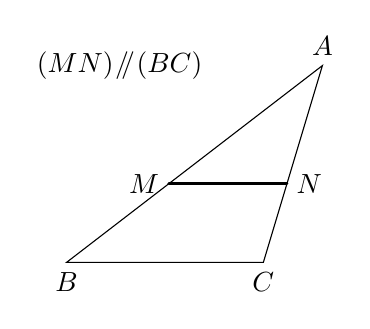
\begin{tikzpicture}[scale=.5,rotate=-90]
                    \coordinate(A)at(0,6.5);
                    \coordinate(A1)at(-0.25,7.75);
                    \coordinate(D)at(5,0);
                    \coordinate(D1)at(5.75,-0.25);
                    \coordinate(E)at(5,5);
                    \path(A)--(E)coordinate[pos=.6](B);
                    \tkzDefLine[parallel=through B](E,D) \tkzGetPoint{i}
                    \tkzInterLL(i,B)(A,D) \tkzGetPoint{C}
                    \draw(A)--(E)--(D)--cycle;
                    \tkzDrawSegment[line width=1pt](B,C)
                    \tkzLabelPoint[above](A){$A$}
                    \tkzLabelPoint[right](B){$N$}
                    \tkzLabelPoint[left](C){$M$}
                    \tkzLabelPoint[below](D){$B$}
                    \tkzLabelPoint[below](E){$C$}
                    \node[right] at(0,-1){\normalsize$(MN)\parallelsum(BC)$};
                \end{tikzpicture} & 
                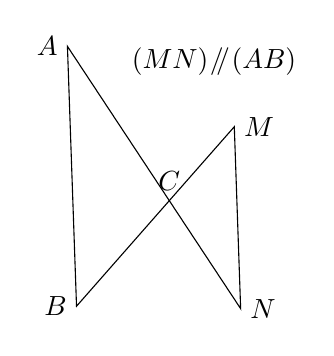
\begin{tikzpicture}[scale=.35,rotate=-30]
                    \coordinate(A)at(0,8);
                    \coordinate(A1)at(-0.25,7.75);
                    \coordinate(D)at(5,0);
                    \coordinate(D1)at(5.75,-0.25);
                    \coordinate(E)at(6,5);
                    \path(A)--(E)coordinate[pos=1.7](B);
                    \tkzDefLine[parallel=through B](A,D) \tkzGetPoint{i}
                    \tkzInterLL(i,B)(E,D) \tkzGetPoint{C}
                    \draw(A)--(E)--(D)--cycle;
                    \draw (E)--(C)--(B)--cycle;
                    \tkzLabelPoint[left](A){$A$}
                    \tkzLabelPoint[right](B){$N$}
                    \tkzLabelPoint[right](C){$M$}
                    \tkzLabelPoint[left](D){$B$}
                    \tkzLabelPoint[above](E){$C$}
                    \node[right] at(2,8.5){\normalsize$(MN)\parallelsum(AB)$};
                \end{tikzpicture} \\
                \end{tblr}\par \medskip 
                \begin{solutionordottedlines}[2.5cm]
                    contenu...
            \end{solutionordottedlines}}
            \part Une paire de chaussure est affichée au prix de $150$~\texteuro. Elle est en promotion et son prix est baissé de $40$~\%. Donner le prix final de l'article. 
            \fullwidth{
                \begin{tblr}{colspec={*4{X[c,m]}}, hlines, vlines}
                    $60$~\texteuro & $75$~\texteuro & $90$~\texteuro & $210$~\texteuro \\
                \end{tblr}\par \medskip 
                \begin{solutionordottedlines}[2.5cm]
                    contenu...
            \end{solutionordottedlines}}
        \end{parts}
        
        \newpage 
        \question[4]
        Le Futuroscope est un parc de loisir situé dans la Vienne. L'année $2019$ a enregistré $1.9$~million de visiteurs.
        \medskip
        \begin{parts}
            \part Combien aurait-il fallu de visiteurs en plus en $2019$ pour atteindre $2$ million de visiteurs~?
%            \begin{solutionordottedlines}[1.5cm]
%                Il aurait fallu $0.1$ million de visiteurs en plus soit $100 \ 000$ visiteurs en plus.
%            \end{solutionordottedlines}
            \part L'affirmation "Il y a eu environ $5200$ visiteurs par jour en $2019$" est-elle vraie~? Justifier la réponse.
%            \begin{solutionordottedlines}[1.5cm]
%                $\frac{1 \ 900 \ 000}{365}=5205$ donc c'est vrai.
%            \end{solutionordottedlines}
            \part Un professeur organise une sortie pédagogique au Futuroscope pour ses élèves de troisième. Il veur répartir les $126$ garçons et les $90$ filles par groupes. Il souhaite que chaque groupe comporte le même nombre de filles et le même nombre de garçons. \medskip
            \begin{subparts}
                \subpart Décomposer en produit de facteurs premiers les nombres $126$ et $90$.
%                \begin{solutionordottedlines}[1.5cm]
%                    $126=2\times 3^2\times 7$ \\
%                    $90=2 \times 3^2\times 5$
%                \end{solutionordottedlines}
                \subpart Trouver tous les entiers qui divisent à la fois les nombres $126$ et $90$.
%                \begin{solutionordottedlines}[2cm]
%                    Les entiers divisant à la fois $126$ et $90$ sont $1$, $2$, $3$, $6$, $9$, $18$.
%                \end{solutionordottedlines}
                \subpart En déduire le plus grand nombre de groupes que le professeur pourra constituer. Combien de filles et de garçons y aura-t-il alors dans chaque groupe~?
%                \begin{solutionordottedlines}[2.5cm]
%                    Il pourra faire $18$ groupes qui contiendront alors $7$ garçons et $5$ filles.
%                \end{solutionordottedlines}
            \end{subparts}
            \part Deux élèves de $3^\text{e}$, Marie et Adrien, se souviennent avoir vu en mathématiques que les hauteurs inaccessibles pouvaient être déterminées avec l'ombre. Ils souhaitent calculer la hauteur de la Gyrotour du Futuroscope. \par \medskip Marie se déplace comme indiqué sur la figure ci-dessous, de telle sorte que son ombre coïncide avec celle de la tour. Après avoir effectués plusieurs mesures, Adrien effectue le schéma ci-dessous (le schéma n'est pas à l'échelle) sur lequel les points $A$, $E$ et $B$ ainsi que les points $A$, $D$ et $C$ sont alignés. \par \medskip Calculer la hauteur $BC$ de la Gyrotour.
%            \begin{solutionordottedlines}[8cm]
%                On utilise le théorème de Thalès : $\frac{AD}{AC}=\frac{AE}{AB}=\frac{DE}{BC}$ \\
%                Donc : $BC=\frac{1.6\times 56.25}{2}=45$~m.
%            \end{solutionordottedlines}
            \part Le Futuroscole souhaite poser une tyrolienne du haut de la tour au point $A$. Calculer la longueur de cable nécessaire pour rejoindre les points $A$ et $B$. 
        \end{parts}
        \begin{center}
            \begin{tikzpicture}
                \coordinate[label=below:$A$](A)at(0.5,0.5);
                \coordinate[label=below:$C$](C)at(12.6,0.5);
                \coordinate[label=above:$B$](B)at(12.6,6);
                \coordinate[label=below:$D$](D)at(3.5,0.5);
                \draw[dashed](3.5,1.84)--(3.5,4);
                \coordinate[label=above:$E$](E)at(3.5,1.85);
                \tkzMarkRightAngle[size=0.3](B,C,A)
                \tkzMarkRightAngle[size=0.3](E,D,A)
                \draw[dashed](3.5,1.85)--(4,1.85);
                \draw(A)--(B)--(C)--cycle;
                \draw(D)--(E);
                \tkzLabelSegment[sloped,below](C,B){Gyrotour}
                \tkzLabelSegment[left=-18pt](E,D){Marie}
                \draw[Stealth-Stealth](0.5,-0.1)--(3.5,-0.1);
                \node[below] at (2,-0.1){$2$~m};
                \draw[Stealth-Stealth](3.5,-0.1)--(12.6,-0.1);
                \node[below] at (8.05,-0.1){$54.25$~m};
                \draw[Stealth-Stealth](4,0.5)--(4,1.84);
                \node[right] at (4,1.17){$1.6$~m};
                \draw[-Stealth](13.4,3.2)--(13.4,6);
                \draw[Stealth-](13.4,0.5)--(13.4,2.8);
                \node[rotate=90] at (13.4,3){?};
            \end{tikzpicture}
        \end{center}
        
        \vfill 
        \question[3] Dans cet exercice, le carré $ABCD$ n'est pas représenté en vraie grandeur. \par         
        Aucune justification n'est attendue pour les questions 1. et 2. On attend des réponses justifiées pour la question 3.\par \medskip
        \begin{parts}
            \begin{minipage}[c]{.68\linewidth}
                \part On considère le carré $ABCD$ de centre $O$ représenté
                ci-dessous, partagé en quatre polygones superposables, numérotés
                {\large\protect\textcircled{\small 1}},
                {\large\protect\textcircled{\small 2}},
                {\large\protect\textcircled{\small 3}}, et
                {\large\protect\textcircled{\small 4}}.
                \begin{subparts}
                    \subpart Quelle est l'image du polygone {\large\protect\textcircled{\small 1}} par la symétrie centrale de centre $O$~? \par \medskip
                    \subpart Quelle est l'image du polygone {\large\protect\textcircled{\small 4}} par la rotation de centre $O$ qui transforme le polygone {\large\protect\textcircled{\small 1}} en le polygone {\large\protect\textcircled{\small 2}}~?
                \end{subparts}
            \end{minipage}\hfill
            \begin{minipage}[c]{.28\linewidth}
                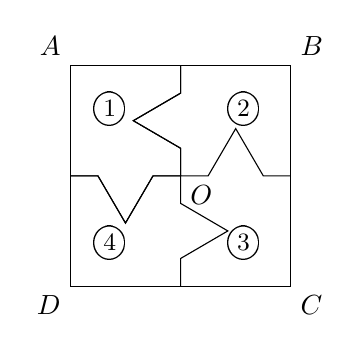
\begin{tikzpicture}
                    \def\motif{\draw(0,1.4)--(0,1.05)--(-0.6,0.7)--(0,0.35)--(0,0)--(0.35,0)--(0.7,0.6)--(1.05,0)--(1.4,0);}
                    \draw(0,0)rectangle(2.8,2.8);
                    \node[above left]at(0,2.8){$A$};
                    \node[above right]at(2.8,2.8){$B$};
                    \node[below right]at(2.8,0){$C$};
                    \node[below left]at(0,0){$D$};
                    \begin{scope}[shift={(1.4,1.4)}]
                        \motif
                    \end{scope}
                    \begin{scope}[shift={(1.4,1.4)},rotate=90]
                        \motif
                    \end{scope}
                    \begin{scope}[shift={(1.4,1.4)},rotate=180]
                        \motif
                    \end{scope}
                    \node at(0.5,2.2){{\large\protect\textcircled{\small 1}}};
                    \node at(2.2,2.2){{\large\protect\textcircled{\small 2}}};
                    \node at(2.2,0.5){{\large\protect\textcircled{\small 3}}};
                    \node at(0.5,0.5){{\large\protect\textcircled{\small 4}}};
                    \node[below right]at(1.4,1.4){$O$};
                \end{tikzpicture}
            \end{minipage}\par \medskip
            \part La figure ci-dessous est une partie de pavage dont un motif de base est le carré $ABCD$ de la question 1.\par            
            Quelle transformation partant du polygone {\large\protect\textcircled{\small 1}} permet d'obtenir le polygone {\large\protect\textcircled{\small 5}}~?
            \def\zig{\def\motif{\draw(0,1.4)--(0,1.05)--(-0.6,0.7)--(0,0.35)--(0,0)--(0.35,0)--(0.7,0.6)--(1.05,0)--(1.4,0);}
                \begin{scope}[shift={(1.4,1.4)}]
                    \motif
                \end{scope}
                \begin{scope}[shift={(1.4,1.4)},rotate=90]
                    \motif
                \end{scope}
                \begin{scope}[shift={(1.4,1.4)},rotate=180]
                    \motif
            \end{scope}}
            \fullwidth{\vspace{-0.5cm}
                \begin{center}
                    \begin{tikzpicture}[scale=1.05]
                        \foreach \n in {0,2.8,5.6,...,16.8} {
                            \foreach \na in {0,2.8,5.6} {
                                \begin{scope}[shift={(\n,\na)}]
                                    \zig
                                \end{scope}
                                \draw(\n,0)--(\n,8.4);
                            }
                        }
                        \draw(16.8,0)--(16.8,8.4);
                        \draw(0,0)--(16.8,0);
                        \draw(0,2.8)--(16.8,2.8);
                        \draw(0,5.6)--(16.8,5.6);
                        \draw(0,8.4)--(16.8,8.4);
                        \node at (0.5,7.7){{\large\protect\textcircled{\small 1}}};
                        \node at(3.3,7.7){{\large\protect\textcircled{\small 5}}};
                        \node[above left] at(0,8.4){$A$};
                        \node[above right]at(2.8,8.4){$B$};
                        \node[below left]at(0,5.6){$D$};
                        \node[below right]at(2.8,5.6){$C$};
                        \node[below right]at(1.4,7){$O$};
                    \end{tikzpicture}
            \end{center}}
            \part On souhaite faire imprimer ces motifs sur un tissu rectangulaire de longueur $315$~cm et de largeur $270$~cm. \par On souhaite que le tissu soit entièrement recouvert par les carrés identiques à $ABCD$, sans découpe et de sorte que le côté du carré mesure un nombre entier de centimètres.
            \begin{subparts}
                \subpart Montrer qu'on peut choisir des carrés de $9$~cm de côté.
                \subpart Dans ce cas, combien de carrés de $9$~cm de côté seront imprimés sur le tissu~?
            \end{subparts}
        \end{parts}
        
        \vfill 
        \question[3] Voici la série des temps exprimés en secondes, et réalisés par des nageuses lors de la finale du $100$~mètres féminin nage libre lors des championnats d'Europe de natation de 2018~:
        \begin{center}
            \begin{tblr}{colspec={*{8}{X[c,m]}}, hlines, vlines}
                $53.23$&$54.04$&$53.61$&$54.52$&$53.35$&$52.93$&$54.56$&$54.07$\\ 
            \end{tblr}
        \end{center}\par \medskip
        \begin{parts}
            \part La nageuse française, Charlotte BONNET, est arrivée troisième à cette finale. Quel est le temps, exprimé en secondes, de cette nageuse ?
            \part Quelle est la vitesse moyenne, exprimée en m/s, de la nageuse ayant parcouru les $100$ mètres en $52,93$ secondes ? Arrondir au dixième près.
            \part Comparer moyenne et médiane des temps de cette série.\par \medskip
            Sur une feuille de calcul, on a reporté le classement des dix premiers pays selon le nombre de médailles d'or lors de ces championnats d'Europe de natation, toutes disciplines confondues~:
            \begin{center}
                \begin{tblr}{colspec={*3{Q[c,m]} *4{X[c,m]}}, hlines, vlines}
                    &A&B &C& D &E &F\\ 
                    1& Rang &Nation &Or 	&Argent &Bronze &Total\\ 
                    2&1		&Russie 		&23	&15 &9 	&47 \\ 
                    3&2		&Grande-Bretagne&13	&12 &9 	&34 \\ 
                    4&3		&Italie 		&8	&12 &19 &39\\
                    5&4		&Hongrie 		&6	&4	&2	&12\\ 
                    6&5		&Ukraine 		&5	&6 	&2 	&13\\ 
                    7&6		&Pays-Bas 		&5	&5 	&2 	&12\\ 
                    8&7		&France 		&4	&2 	&6 	&12\\ 
                    9&8		&Suède 			&4	&0 	&0 	&4\\ 
                    10&9	&Allemagne 		&3	&6 	&10 &19\\
                    11&10	&Suisse 		&1	&0 	&1 	&2\\ 
                \end{tblr}
            \end{center}\par \medskip
            \part Est-il vrai qu'à elles deux, la Grande-Bretagne et l'Italie ont obtenu autant de médailles d'or
            que la Russie ?
            \part Est-il vrai que plus de $35$~\% des médailles remportées par la France sont des médailles d'or ?
            \part Quelle formule a-t-on pu saisir dans la cellule F2 de cette feuille de calcul, avant qu'elle soit
            étirée vers le bas jusqu'à la cellule F11 ?
        \end{parts}
        
        \newpage
        \question[4] Dans cet exercice, $x$ est un nombre strictement supérieur à $3$.\par        
        On s'intéresse aux deux figures géométriques dessinées ci-dessous~:
        \begin{itemize}[label=\textbullet]
            \item un rectangle dont les côtés ont pour longueurs $x-3$ et $x+7$.
            \item un carré de côté $x$.
        \end{itemize}
        
        \begin{center}
            \begin{tikzpicture}[scale=0.9]
                \draw(0,0)rectangle(5,2);
                \draw(7,0)rectangle(11,4);
                \node[left] at (0,1){$x-3$};
                \node[below] at (2.5,0){$x+7$};
                \node[left]at(7,2){$x$};
                \node[below]at(9,0){$x$};
            \end{tikzpicture}
        \end{center}
        
        \begin{parts}
            \part Quatre propositions sont écrites ci-dessous :  \par 
            Recopier sur la copie celle qui correspond à l'aire du carré. On ne demande pas de justifier.
            \begin{center}
                \begin{tblr}{colspec=*4{X[c,m]}, hlines, vlines}
                    $4x$&$4+x$&$x^2$&$2x$\\
                \end{tblr}
            \end{center}
            \part  Montrer que l'aire du rectangle est égale à $x^2 + 4x - 21$.
            \part On a écrit le script ci-dessous dans Scratch.\par 
            On veut que ce programme renvoie l'aire du rectangle lorsque l'utilisateur a rentré une valeur de $x$ (strictement supérieure à $3$).\par 
            Écrire sur la copie les contenus des trois cases vides des lignes 5, 6 et 7, en précisant les numéros de lignes qui correspondent à vos réponses.\par 
            \hspace*{2cm}
            \begin{scratch}[num blocks]
                \blockinit{Quand la touche\selectmenu{espace} est pressée}
                \blocklook{demander \ovalnum {combien vaut x ?} et attendre}
                \blockvariable{mettre \selectmenu{x} à \ovalsensing{réponse}}
                \blockvariable{mettre \selectmenu{R} à \ovalvariable{x}*\ovalvariable{x}}
                \blockvariable{ajouter \ovalnum{}*\ovalvariable{x} à \ovalvariable{R}}
                \blockvariable{ajouter \ovalnum{} à \ovalvariable{R}}
                \blocklook{dire \ovaloperator{regrouper \ovalnum{L'aire du rectangle est }et \ovalnum{}} pendant \ovalnum{2} secondes}
            \end{scratch}\\
            
            \part On a pressé la touche espace puis saisi le nombre $8$. Que renvoie le programme ?
            \part Quel nombre $x$ doit-on choisir pour que l'aire du rectangle soit égale à l'aire du carré ?\par 
            \emph{Toute trace de recherche, même non aboutie, sera prise en compte.} 
        \end{parts}
        
            
    \end{questions}
    
\end{document}
